% 2024年北京高考数学第20题解析图1：曲线与割线分析
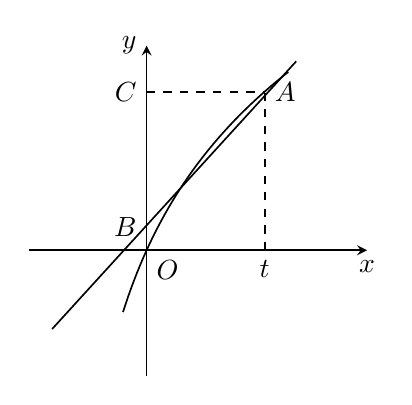
\begin{tikzpicture}[>=stealth,line width=0.6pt,font=\normalsize]
  \draw[->] (-1.5,0) -- (2.8,0) node[below] {$x$};
  \draw[->] (0,-1.6) -- (0,2.6) node[left] {$y$};
  \node[below right] at (0,0) {$O$};

  % 曲线 y = ln(x+1) 或类似凹函数
  \draw[domain=-0.3:1.8,smooth,samples=40] plot (\x, {2.2*ln(\x+1)});

  % 点 A(t, f(t)) 与辅助线
  \coordinate (A) at (1.5,2.01);
  \coordinate (B) at (0,0.3);
  \coordinate (C) at (0,2.01);

  \draw[dashed] (1.5,0) node[below] {$t$} -- (A);
  \draw[dashed] (C) node[left] {$C$} -- (A);

  % 割线 AB
  \draw (-1.2,-1.0) -- (1.9,2.4);

  \node[right] at (A) {$A$};
  \node[left] at (B) {$B$};
\end{tikzpicture}
